\documentclass[12pt]{kiarticle} 
\graphicspath{{pictures/}}
\DeclareGraphicsExtensions{.pdf,.png,.jpg,.eps}
\usepackage{indentfirst}
\newcommand{\del}{\ensuremath{\delta}}
\newcommand{\co}{\ensuremath{\mathrm{const}}}
\newcommand{\D}{\ensuremath{\mathcal{D}}}
\newcommand{\spdd}[2]{\left( \frac{\partial #1}{\partial #2} \right)}
\newcommand{\Dd}[4]{\frac{\partial \left( #1, #2\right) }{\partial \left( #3, #4\right)}}
%%%
\fancyhead[L]{Вопрос по выбору --- термодинамика, 2017\hfil}
\fancyhead[R]{\hfil Иванов Кирилл, 625 группа }



\begin{document}

\begin{titlepage}
	\begin{center}
		\large 	Московский физико-технический университет \\
		Факультет общей и прикладной физики \\
		\vspace{0.2cm}
		
		\vspace{4.5cm}
		Вопрос по выбору во 2 семестре \\ \vspace{0.2cm}
		\large (Общая физика: термодинамика) \\ \vspace{0.2cm}
		\LARGE \textbf{Основы и аксиоматика термодинамики оригинальным путём}
	\end{center}
	\vspace{2.3cm} \large
	
	\begin{center}
		Автор: \\
		Иванов Кирилл,
		625 группа
		\vspace{10mm}
		
		Семинарист: 
		
		Слободянин Валерий Павлович
		
		
	\end{center}
	
	\begin{center} \vspace{50mm}
		г. Долгопрудный \\
		 2017 год
	\end{center}
\end{titlepage}

%%%%%%%%%%
%%%%%%%%%%
%%%%%%%%%%%%%%%%%%%%%%%%%%%%%%%%%%%

\section{Введение}

В курсе термодинамики, изучаемом в МФТИ, постулируют сначала так называемое "<нулевое"> и затем первое начала термодинамики, а затем, изучая тепловые машины и циклы, приходят ко второму началу термодинамики. В процессе такого перехода весьма естественно формируется определение \textbf{энтропии} как приведённого тепла: 

\begin{equation}\label{entmipt}
 dS = \dfrac{\del Q}{T}
\end{equation}

Впоследствии с помощью этого получается обобщение первого начала термодинамики в виде $ TdS = dU + \del A $. 

Мы же попробуем ввести понятие энтропии немного по-другому, опираясь на другие понятия.

\section{Вывод энтропии}

\subsection{Определение условных параметров} \label{ifTS}

Рассмотрим произвольный сосуд с некоторым газом. Весьма естественно определить такие макропараметры, как \textit{давление} $ P $ и \textit{объем} $ V $ из чисто логических и механических соображений. Введём также понятие \textit{условной температуры} $ \tau $ как некого третьего параметра нашей системы и будем считать его "<мерой нагретости тела"> (понимая, однако, наличие и более объективного смысла температуры, на котором мы не будем останавливаться в данной работе). 

\begin{wrapfigure}{l}{0.35\linewidth} 
	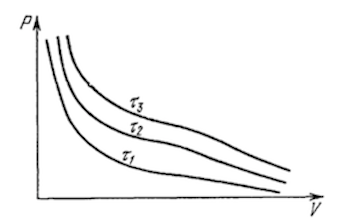
\includegraphics{tempdef}
	\caption{Семейство изотерм с температурой $ \tau_i $}
\end{wrapfigure}

Определив \textit{термостат} как тело с бесконечно большой теплоёмкостью, поместим туда наш газ. Зафиксировав в термостате этот параметр, будем изменять $ P $ и $ V $, и так сделаем для разных температур. Опыты показывают, что для каждой температуры можно построить кривую (\textit{изотерму}) на плоскости $ PV $, которые не будут пересекаться, и при нормальных условиях будут приближённо иметь вид гипербол. 

Тогда такой газ мы назовём \textit{идеальным}, а условная температура $ \tau = \tau (P, V) $ будет являться функцией состояния системы. Кроме того, для уравнения состояния будет справедливо следующее:

\begin{equation}\label{defte}
PV = \co \te \tau (P, V) = \tau (PV)
\end{equation}

Так можно сформулировать \textbf{принцип температуры} о существовании функции состояния, остающейся неизменной при любом процессе на изотерме (в термостате).

\begin{wrapfigure}{l}{0.34\linewidth} 
	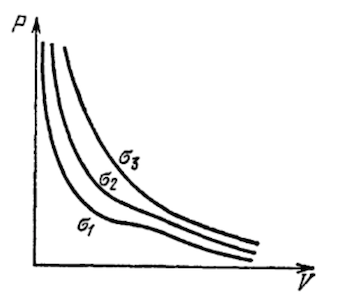
\includegraphics{entdef}
	\caption{Семейство адиабат с энтропией $ \sigma_i $}
\end{wrapfigure}

Теперь определим \textit{адиабат} как абсолютно теплонепроницаемое тело и получим другое семейство кривых с параметром \textit{условной энтропии}. Так как они не пересекаются, то $ \sigma = \sigma (P, V) $ тоже однозначная функция состояния системы, и можно сформулировать \textbf{принцип энтропии}. Для введённого выше идеального газа  уравнение состояния имеет вид (полученный опытным путем)

\begin{equation}\label{defent}
PV^\gamma = \co \te \sigma (P, V) = \sigma (PV^\gamma)
\end{equation}

где $ \gamma > 1 $ --- \textit{показатель адиабаты}. Таким образом, обозначив константы из \eqref{defte} и \eqref{defent} за $ x, y $ соответственно, мы получаем однозначное решение этой системы в виде

\begin{equation}\label{xy}
P = \left( \dfrac{x^\gamma}{y} \right)^\frac{1}{\gamma -1}, \quad V = \left (\dfrac{y}{x} \right )^\frac{1}{\gamma -1} 
\end{equation}

\subsection{Абсолютные параметры}

Результаты, полученные в \eqref{xy}, также показывают нам очень важное свойство --- каждая адиабата и каждая изотерма пересекаются в одной и только одной точке плоскости $ PV $. Тогда мы получаем, что соотношение между парами параметров газа $ P, V $ и $ \tau, \sigma $ является \textbf{взаимно однозначным}, и плоскость $ PV $  эквивалентна $ \tau \sigma $-плоскости. Рассмотрим это поподробнее.

Переход одной плоскости в другую эквивалентен следующему переходу элементарных площадей: 

\begin{equation}\label{}
dP dV \st \D d\tau d\sigma
\end{equation}

где $ \D  = \pdd{(P, V)}{(\tau, \sigma)} $ --- \textit{якобиан}. Тогда естественно положить $ \D = 1 $ для полного равноправия наших плоскостей. Эта нормировка позволяет выбрать определённые температурные и энтропийные шкалы, и отсчитываемые по ним величины мы будем называть уже \textit{абсолютными} температурой $ T $ и энтропией $ S $. Получаем:

\begin{equation}\label{D}
\D  = \pdd{(P, V)}{(T, S)} = 1
\end{equation}

Пользуясь вышевведенными обозначениями и считая $ T = T(x), S = S(y) $, мы воспользуемся формулой произведения якобианов: $  \pdd{(P, V)}{(\tau, \sigma)} = 1 \ekv  \pdd{(T, S)}{(x, y)} \pdd{(x, y)}{(P, V)} = 1 \te$

\begin{equation}\label{DD}
\begin{vmatrix}
\pdd{T}{x} & \pdd{T}{y} \\
\pdd{S}{x} & \pdd{S}{y} \\
\end{vmatrix} 
\x
\begin{vmatrix}
\pdd{x}{P} & \pdd{x}{V} \\
\pdd{y}{p} & \pdd{y}{V} \\
\end{vmatrix}
=
\left( \dfrac{dT}{dx} \dfrac{dS}{dy} - 0\right) \left( V\x \gamma PV^{\gamma - 1} - P\x V^\gamma\right) = T' S' y(\gamma - 1) = 1
\end{equation}

Так мы получаем следующее соотношение, в котором левая часть является функцией от $ x $, а правая от $ y $:

\begin{equation}\label{T'S'}
T' = \dfrac{1}{S'y(\gamma - 1)}
\end{equation}

Тогда эти части равны одной и той же константе, которую мы обозначим за $ \frac{1}{R} $:

\begin{equation}\label{R}
T' = \dfrac{dT}{dx} = \dfrac{1}{R}, \quad S' = \dfrac{dS}{dy} = \dfrac{R}{\gamma - 1} \dfrac{1}{y}
\end{equation}

Проинтегрируем эти уравнения:
\begin{equation}\label{TS}
\sys{
&T = \dfrac{x}{R} + C_T = \dfrac{PV}{R}  + C_T \\
&S = \dfrac{R}{\gamma -1} \ln y + C =  \dfrac{R}{\gamma -1} \ln PV^\gamma + C
}
\end{equation} 

Где, конечно, $ C_T, C $ --- константы интегрирования. Для удобства превратим величину под логарифмом в безразмерную, выбрав $ C = S_0 - \frac{R}{\gamma -1} \ln P_0V^\gamma_0$:

\begin{equation}\label{S}
S - S_0 = \dfrac{R}{\gamma -1} \ln  \dfrac{PV^\gamma}{P_0V_0^\gamma} = \dfrac{R}{\gamma -1} \ln \dfrac{(T - C_T) V^{\gamma - 1}}{(T_0 - C_T) V^{\gamma -1 }_0} = \dfrac{R}{\gamma -1} \ln \frac{(T - C_T)^\gamma P^{1 - \gamma}}{(T_0 - C_T)^\gamma P_0^{1 -\gamma}}
\end{equation}

Так мы получили соотношения для температуры и энтропии, опираясь на введённые в параграфе \ref{ifTS} утверждения. Постоянная $ R $ будет определять лишь масштаб наших шкал, и выбрав ее равной $ R = 8,31 $ Дж/К$ \x $моль, получим шкалу Кельвина для температуры. 

\subsection{Плоскость TS}

\begin{wrapfigure}{l}{0.45\linewidth} 
	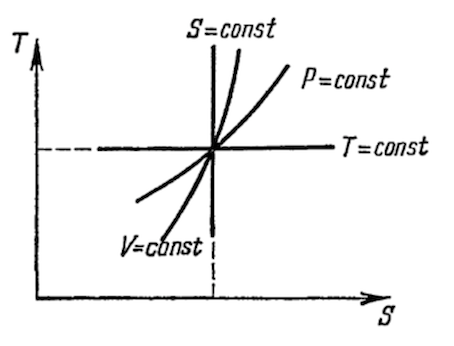
\includegraphics{TS}
	\caption{Изопроцессы на плоскости $ TS $}
	\label{GrafTS}
\end{wrapfigure}

Пользуясь первым уравнением из \eqref{TS} и первым равенством из \eqref{S}, мы получаем систему:

\begin{equation}\label{sysTS}
\sys{
&PV = RT \\
&PV^\gamma = \co \; e^{(\gamma - 1)\frac{S}{R}}
}
\end{equation}

Тогда, выражая из первого давление для изохорного и объем для изобарного процессов, второе уравнение будет иметь следующий вид:

\begin{equation}\label{}
\sys{
& V = \co \te T = T_1(V) \; e^{(\gamma - 1)\frac{S}{R}} \\
& P = \co \te T = T_2(P) \; e^{(\gamma - 1)\frac{S}{\gamma R}} \\
}
\end{equation}

Где $ T_1(V), T_2(P) $ --- функции от объёма и давления, равные константам при фиксированных аргументах. Это и позволяет нам получить график всех знакомых изопроцессов на рис.\ref{GrafTS}. 

%%%%%%%%%%%%%%%%%%%%%%%%%%
%%%%%%%%%%%
%%%%%%%%%
%%%%%%%%%%%



%%%%%%%%%%%%%%%%%%%%%%%%%%
%%%%%%%%%%%
%%%%%%%%%
%%%%%%%%%%%

%\newpage 
%\section{Интересные свойства}
%
%Вернемся теперь к стандартному представлению термодинамики и обратим внимание на некоторые интересные особенности энтропии и второго начала термодинамики.
%
%\subsection{Статистическая энтропия}
%
%Вообще понятие времени и его направленность в термодинамике очень важны. В самом деле, это следует из формулировки Клазиуса 2 начала термодинамики и понятия необратимых процессов.
% 
% \begin{equation}\label{}
% S = k \ln G
% \end{equation}
% 
% Вводя энтропию через статистический вес, мы получаем, что она является как бы "<мерой хаоса"> системы. Действительно, чем больше энтропии, тем больше статистический вес системы, т.е. тем большее число возможных состояний система может иметь. С этой точки зрения можно понимать возможность системы принять большее число состояний за неупорядоченность и недетерминируемость, т.е. за "<хаос">.
%
%Верен \textbf{закон неубывания энтропии}: среди всех направлений эволюции системы предпочтительным оказывается то, при котором вероятность конечного состояния оказывается наибольшей. Т.е. с наибольшей вероятностью $ \frac{dS}{dt} \geq 0 \te S\uparrow $ --- монотонно не убывает (за исключением флуктуаций).
%
%\subsection{Термодинамическая стрела времени}
%
%
%Британский ученый Стивен Хокинг в своей знаменитой книге "<Краткая история времени"> выделял весьма интересную вещь: \textbf{стрелу времени}. Суть этого понятия в том, что, несмотря на последовавшее после СТО и ОТО Эйнштейна объединение пространства-времени в единое четырехмерное целое, временная ось все же немного отличается от пространственных хотя бы тем, что у нее есть строгая направленность. 
%
%А именно, существует три стрелы времени: \textbf{термодинамическая} (указывающая направление времени, в котором возрастает беспорядок), \textit{психологическая} (направление, в котором мы помним прошлое, а не будущее) и \textit{космологическая} (направление, в котором Вселенная расширяется, а не сжимается). И все они направлены в одном направлении. 
%
%Рассмотрим подробнее термодинамическую. Она говорит нам о том, что всегда система с высокой степенью порядка с течением времени будет сохранять свое положение либо перейдет в состояние беспорядка (переформулировка закона неубывания энтропии).
%
%Предположим обратное, что законы природы предусматривают, что развитие Вселенной из любого состояния заканчивается в состоянии высокого порядка. Очевидно, что на ранних стадиях Вселенная скорее всего находилась в состоянии беспорядка, тогда получается, что с течением времени беспорядок уменьшается, что является противоречием. Если бы мы жили в такой Вселенной, то мы бы наблюдали, как осколки упавшей со стола чашки прыгают и склеиваются обратно! 
%
%По мнению исследовавшего этот вопрос Хокинга, психологическая стрела времени этих людей должна быть направлена наоборот -- из будущего в прошлое, т.е. они должны помнить события в будущем, а не в прошлом. Увидев разбитую чашку, они должны вспомнить, как она стоит на столе (в будущем), но когда она из-за уменьшения беспорядка оказывается на столе оказывается на столе, они бы не помнили, как она лежит на полу. 
%
%\subsection{Квантовый демон Максвелла}
%
%\begin{wrapfigure}{l}{0.58\linewidth} 
%	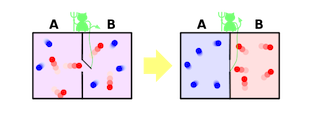
\includegraphics{demon}
%	\caption{Классический демон Максвелла}
%	\label{}
%\end{wrapfigure}
%
%Еще в XIX веке был известен парадокс \textbf{демона Максвелла}. Мысленный эксперимент состоит в следующем: предположим, сосуд с газом разделён непроницаемой перегородкой на две части: правую и левую. В перегородке есть отверстие с устройством (так называемый демон Максвелла), которое позволяет пролетать быстрым (горячим) молекулам газа только из левой части сосуда в правую, а медленным (холодным) молекулам — только из правой части сосуда в левую. Тогда через большой промежуток времени «горячие» (быстрые) молекулы окажутся в правом сосуде, а «холодные» останутся в левом.
%
%Таким образом, получается, что демон Максвелла позволяет нагреть правую часть сосуда и охладить левую без дополнительного подвода энергии к системе. Энтропия для системы, состоящей из правой и левой части сосуда, в начальном состоянии больше, чем в конечном, что противоречит термодинамическому принципу неубывания энтропии в замкнутых системах.
%
%Парадокс разрешается, если рассмотреть замкнутую систему, включающую в себя демона Максвелла и сосуд. Для функционирования демона Максвелла необходима передача ему энергии от стороннего источника. За счёт этой энергии и производится разделение горячих и холодных молекул в сосуде, то есть переход в состояние с меньшей энтропией. 


%%%%%%%%%%
%%%%%%%%%%
%%%%%%%%%%%%%
%%%%%%%%%%%%%%
%%%%%%%%%%%%%%
%%%%%%%%%%%%%%
%%%%%%%%%%%%%%%%

\section{Термодинамические потенциалы}

Обратимся к механической аналогии работы, представив элементарную работу как убыль некой функции --- потенциала силы $ f $ (потенциальной энергии):

\begin{equation}\label{}
\del A = fdx = -dU(x) \te f = -\pdd{U}{x}
\end{equation}

В термодинамике же роль силы и координаты играют давление $ P $ и объем $ V $ соответственно. Тогда введём некий \textit{термодинамический потенциал} так, чтобы его производная по объёму, взятая с противоположным знаком, равнялась давлению. 

Потребуем, чтобы такой потенциал был функцией состояния газа (т.е. однозначно определялся в зависимости от своих параметров), и рассмотрим частные случаи.

\subsection{Адиабатический процесс}

Обозначим за \textit{адиабатический потенциал} $ U $ и запишем работу в адиабатическом процессе (т.е. $ S = \co $):

\begin{equation}\label{U_S}
\del A_S = P dV_S = - dU_S
\end{equation}

Очевидным обобщением на произвольный процесс является добавка члена, зависящего от изменения энтропии:

\begin{equation}\label{U}
dU = - PdV + \al dS
\end{equation}

По математическому свойству полного дифференциала получаем:

\begin{equation}\label{}
\s{\pdd{\al}{V}}_S = - \s{\pdd{P}{S}}_V
\end{equation}

Запишем это в виде равенства якобианов и воспользуемся его свойствами:

\begin{equation}\label{}
\pdd{(\al, S)}{(V, S)} = \pdd{(P, V)}{(V, S)} \te \pdd{(\al, S)}{(P, V} = 1
\end{equation}

Тогда умножим это равенство на знакомый нам якобиан $ \D  = \pdd{(P, V)}{(T, S)} $, равный единице согласно \eqref{D}, и применим формулу произведения якобианов:

\begin{equation}\label{}
\pdd{(\al, S)}{(P, V} \x  \pdd{(P, V)}{(\tau, \sigma)} = 1 \te \pdd{(\al, S)}{(T, S)} = \s{\pdd{\al}{T}}_S = 1
\end{equation}

Отсюда мы можем найти вид функции $ \al $, проинтегрировав последнее соотношение:

\begin{equation}\label{}
\al = T + \varphi(S)
\end{equation}

где $ \varphi(S) $ --- произвольная функция от энтропии. Разумеется, сам потенциал $ U $ определятся из \eqref{U} с точностью до члена $ \int \varphi(S)dS $, что позволяет быть верным исходному равенству \eqref{U_S}. Мы зададим нормировку для $ U $, определив $ \varphi(S) \equiv 0 \te \al = T $. Тогда получаем итоговую формулу для адиабатического потенциала:

\begin{equation}\label{U =}
dU = TdS - PdV
\end{equation}

Отсюда мы видим, что это функция от энтропии и объёма, и производные по этим аргументам соответственно равны 

\begin{equation}\label{}
T = \spdd{U}{S}_V, \quad P = \spdd{U}{V}_S
\end{equation}

\subsection{Изотермический процесс}

Абсолютно аналогично введём \textit{изотермический потенциал} $ F $ как $ \del A_T = P dV_T = - dF_T $, обобщением чего является соотношение

\begin{equation}\label{F}
dF = -PdV + \beta dT
\end{equation}

Опять перепишем это через якобианы: 

\begin{equation}\label{}
\spdd{\beta}{V}_T = - \spdd{P}{T}_V , \te \Dd{\beta}{T}{V}{T} = \Dd{P}{V}{V}{T} ,  \te \Dd{\beta}{T}{P}{V} = 1
\end{equation}

Умножим на якобиан из \eqref{D}:

\begin{equation}\label{}
\Dd{\beta}{T}{T}{S} = -\spdd{\beta}{S}_T = 1 \te \beta = -S + \psi(T)
\end{equation}

Отнормировав функцию $ \beta $ выбором $ \psi(T) \equiv 0 \te \beta=-S $, мы получаем итоговую формулу для изотермического потенциала:

\begin{equation}\label{F =}
dF = - SdT - PdV
\end{equation}

Отсюда мы видим, что это функция от температуры и объёма, и производные по этим аргументам соответственно равны 

\begin{equation}\label{}
S = -\spdd{F}{T}_V, \quad P = - \spdd{F}{V}_T
\end{equation}

Несложно получить простую связь между введёнными потенциалами вычитанием формулы \eqref{F =} из \eqref{U =}:

\begin{equation}\label{}
dU - dF = TdS + SdT \te d(U - F) = d(TS) \te F = U - TS
\end{equation}

Константа интегрирования выбрана равной нулю. 


%%%%%%%%%%%%
%%%%%%%%%%%%
%%%%%%%%%%%%
%%%%%%%%%%%%
%%%%%%%%%%%%

\section{Энергия и теплоёмкость}

Определим \textit{внутреннюю энергию} системы как полную минус кинетическую и потенциальную. Тогда сформулируем \textbf{закон сохранения энергии} в виде возможности изменения внутренней энергии работой $ \del A $или подведением тепла $ \del Q $  (где под \textit{теплом} мы будем понимать энергию, переданную через тепловой контакт):

\begin{equation}\label{E}
dE_{\text{внутр}} = \del Q - PdV
\end{equation}

Заметим при этом, что в адиабатическом процессе передача тепла невозможна, т.е. верно равенство $ E_{\text{внутр}} \equiv U $.

Из этого следует, что равенства \eqref{E} и \eqref{U =} определяют одну и ту же величину, тогда получаем классическое равенство 

\begin{equation}\label{Q}
\del Q = TdS
\end{equation}

Определим также теплоёмкость как 

\begin{equation}\label{}
C = \dfrac{\del Q}{dT}
\end{equation}

Тогда из \eqref{Q} следует естественные понятия теплоёмкости при постоянном объёме и давлению:

\begin{equation} \label{CVP}
C_V = T \spdd{S}{T}_V, \quad C_P = T \spdd{S}{T}_P
\end{equation} 

Теперь мы можем доказать для идеального газа классические утверждения. Продифференцируем \eqref{S} и подставим в формулы для \eqref{CVP}, получая

\begin{equation}\label{}
C_V = \dfrac{R}{\gamma - 1} \dfrac{T}{T - C_T}, \quad C_P = \dfrac{\gamma R}{\gamma - 1} \dfrac{T}{T - C_T} 
\end{equation}

Отсюда понятно, что так как для ИГ эти величины есть константы, то зависимость от $ T $ уходит при $ C_T = 0 $. Тогда получаем известные формулы:

\begin{equation}\label{}
C_V = \dfrac{R}{\gamma - 1},  \quad C_P = \dfrac{\gamma R}{\gamma - 1}, \te \gamma = \dfrac{C_P}{C_V}, \quad C_P - C_V = R
\end{equation}


\section{Вывод}

Таким образом, мы получили все знакомые из курса термодинамики МФТИ понятия совершенно другим способом, опираясь на различные экспериментальные данные и построив другую систему аксиом --- принцип температуры и энтропии, равенство \eqref{D} и  закон сохранения энергии.






\section*{Список литературы}

\begin{enumerate}
	
	\item Ю.Б. Румер, М.Ш. Рывкин --- "<Термодинамика, статистическая физика и кинетика">, издание второе ---  издательство "<Наука">, главная редакция физико-математической литературы --- Москва, 1977 
	
	\item Кириченко Н.А. "<Термодинамика и статистическая и молекулярная физика: Учеб. пособие для вузов, 4-е изд., испр. и доп. --- М.: Физмат-книга, 2012. 
	
\end{enumerate}














\end{document}
	
